\documentclass[conference]{IEEEtran}
\IEEEoverridecommandlockouts

\usepackage{amsmath,amssymb,amsfonts}
\usepackage{algorithm}
\usepackage{algpseudocode}
\usepackage{graphicx}
\usepackage{booktabs}
\usepackage{cite}
\usepackage{url}

% stfloats lets a double-column float sit at the BOTTOM of a page. Without it
% \begin{table*} and \begin{figure*} may only go at the top, so once one wide
% float is deferred the rest queue behind it: an earlier build stranded Table I
% and Fig. 2 on the references page and Figs. 3 and 4 on the page after. If it
% ever misbehaves, delete this line and change the [!tb] on the three wide
% floats back to [!t]; the paper still compiles, just less tidily.
\usepackage{stfloats}

% Three of the floats span both columns (Table I, Figs. 2 and 3). With the
% stock fractions LaTeX refuses to place a wide float on a page that already
% carries one and defers it, which is what strands figures at the end. These
% are the usual conservative loosenings, not float-page settings.
\setcounter{topnumber}{3}
\setcounter{totalnumber}{4}
\renewcommand{\topfraction}{0.9}
\renewcommand{\bottomfraction}{0.6}
\renewcommand{\textfraction}{0.08}
\renewcommand{\floatpagefraction}{0.7}

\def\BibTeX{{\rm B\kern-.05em{\sc i\kern-.025em b}\kern-.08em T\kern-.1667em\lower.7ex\hbox{E}\kern-.125emX}}

\begin{document}

% Line breaks are set by hand and measured: at the 23.9 pt title face the
% usable width is 516 pt, and these three lines come out 418, 304 and 428 pt.
% Do not merge them. Putting "Backdoor-Resilient" on the first line makes it
% 620 pt, and LaTeX then rewraps the whole title into four lines with
% "Networks" stranded on its own.
\title{Receiver-Domain Behavioral Probing for\\
Backdoor-Resilient Federated\\
GPS Spoofing Detection in UAV Networks}

% Three stacked lines, matching the reference ICC paper: names, then one shared
% affiliation, then the emails. No superscript markers, since the affiliation
% is common to all authors.
\author{\IEEEauthorblockN{Will Jedrzejczak, Cole Walther, Dilpreet Gill, and Khalid Hasan}
\IEEEauthorblockA{Department of Computer Science, James Madison University, Harrisonburg, VA, USA\\
wjd@gatech.edu, \{walthecp, gillds\}@dukes.jmu.edu, dwtn6r@jmu.edu}
}

\maketitle

\begin{abstract}
Federated learning lets a UAV fleet train a shared GPS spoofing detector
without raw receiver data leaving any aircraft, and several recent UAV-FL
designs weight each client by the validation accuracy it reports about itself.
We show this self-report is an exploitable attack lever: two compromised
clients of ten that poison part of their data, scale their updates, and inflate
their reported accuracy raise backdoor lift to $+0.3036$, higher than the same
attack achieves without lying. We propose receiver-domain behavioral probing,
in which the coordinator evaluates every submitted model on counterfactual
spoofed samples built by driving each discriminative GPS feature to a benign
value, weighting clients by what their models do rather than what they claim.
Under independent and identically distributed clients this reduces
attacker-induced lift to $-0.0265$, statistically indistinguishable from an
honest fleet, while attributing the attack to the specific compromised
aircraft. Unlike Byzantine-robust aggregation it needs no estimate of how many
clients are compromised: when the true count exceeds the configured value,
Multi-Krum degrades from $+0.0061$ to $+0.2837$ while ours stays near baseline.
Evaluation uses one public single-receiver dataset partitioned into simulated
clients; we also report where the mechanism fails, under strong client
heterogeneity.
\end{abstract}

\begin{IEEEkeywords}
federated learning, UAV networks, GPS spoofing, backdoor attacks, robust aggregation, wireless security
\end{IEEEkeywords}

\section{Introduction}

Unmanned aerial vehicle (UAV) fleets used for disaster response, infrastructure
inspection, and search and rescue navigate primarily by GPS, often beyond
visual line of sight~\cite{mekdad2023survey}. Because satellite signals are
openly broadcast and unauthenticated for civil use, an attacker can transmit a
counterfeit signal stronger than the genuine one and displace an aircraft's
perceived position without any physical access. Detecting spoofing on board is
therefore a safety requirement rather than a convenience.

Federated learning (FL)~\cite{mcmahan2017communication} is an attractive fit:
each UAV trains a local detector on the signals it observes and shares only
model parameters, so raw receiver data never leaves the aircraft and the
wireless link is not saturated exactly when it is under
attack~\cite{udin2025federated}. Recent UAV-FL systems go further and weight
each client by a quality metric. Chai \emph{et
al.}~\cite{chai2025navigation} assign weight from each client's own reported
detection performance; Ud Din \emph{et al.}~\cite{udin2025federated} weight by
behavioral and contribution-frequency metrics; Mowla \emph{et
al.}~\cite{mowla2020federated} prioritize client groups for FANET jamming
detection. All three assume the reported quantity is truthful, as does the
wider reputation- and contribution-weighted
literature~\cite{kang2019incentive,kairouz2021advances}.

\textbf{The gap.} That assumption is the vulnerability. A coordinator that
cannot inspect client data cannot verify a client's claim about itself, so a
metric introduced to improve robustness becomes a second adversarial lever
alongside the model update. The FL security literature was developed against
different targets: model-replacement backdoors assume plain
FedAvg~\cite{bagdasaryan2020backdoor}, local model poisoning targets
Byzantine-robust rules~\cite{fang2020local,blanchard2017machine,yin2018byzantine},
and the most effective known backdoor defenses inspect client data
distributions~\cite{nguyen2024backdoor,mothukuri2021survey}, which a
privacy-preserving UAV deployment does not expose. None evaluates an
aggregation rule that trusts a self-reported metric.

\textbf{Positioning against root-of-trust defenses.} The closest prior work is
FLTrust~\cite{cao2021fltrust}, which shares our premise that the server should
bootstrap trust from a small clean root set rather than believe a client. The
difference is what is measured. FLTrust scores a client by the \emph{direction}
of its update relative to a server update computed on that root set, a global
statistic over the whole parameter vector that a backdoor confined to a small
subspace barely perturbs. We instead score a client by \emph{what its submitted
model does} on counterfactual receiver-domain probes: spoofed samples whose
individual GPS features are overwritten with benign values. This yields
per-client attribution rather than a weighting alone, needs no knowledge of
which probed feature carries the trigger, and under IID conditions needs no
estimate of how many clients are compromised. We do not claim dominance over
every defense; our own results show Multi-Krum is highly competitive in the
nominal setting.

\textbf{Contributions.}
\begin{itemize}
\item We formulate and empirically demonstrate an attack in which compromised
UAV clients exploit self-reported accuracy as an aggregation lever, raising
backdoor lift from $+0.2415$ to $+0.3036$ and making the weighted rule worse
than no weighting at all.
\item We propose receiver-domain behavioral probing, a trust mechanism that
evaluates submitted models on counterfactual spoofed samples across every
discriminative receiver feature and never reads a client-reported metric,
making accuracy inflation inert by construction.
\item We evaluate against seven published aggregation rules on one pipeline,
and identify the operating envelope: the mechanism needs no attacker-count
parameter, generalizes across trigger features, attributes the attack to
individual aircraft, and cannot be evaded by a defense-aware adversary without
that adversary destroying its own backdoor; but cohort-relative suspicion
degrades under client heterogeneity, where the robust-aggregation backstop
carries the protection.
\end{itemize}

\section{System and Threat Model}

\subsection{Federated Detection}

Let $\mathcal{U}=\{U_1,\dots,U_N\}$ be $N$ UAV clients, each holding a private
set $\mathcal{D}_i$ of per-epoch GPS receiver observations labeled authentic or
spoofed. At round $t$ the coordinator broadcasts global parameters
$\omega(t)$; each client runs $I$ local steps,
\begin{equation}
\omega_i^{j+1}(t)=\omega_i^{j}(t)-\eta\nabla f_i\!\left(\omega_i^{j}(t);\xi_i^{j}(t)\right),
\label{eq:local}
\end{equation}
where $j$ indexes the local step, $\xi_i^j(t)$ a minibatch drawn from
$\mathcal{D}_i$ and $\eta$ the local learning rate. Each client returns
$\omega_i^{I}(t)$ together with a self-computed validation accuracy
$\mathrm{Acc}_i$, measured on a held-out split of its own data. Following the
accuracy-weighted design of~\cite{chai2025navigation}, the coordinator forms
$\lambda_i=\mathrm{Acc}_i/\sum_k \mathrm{Acc}_k$ and updates
\begin{equation}
\omega(t+1)=\omega(t)+\sum_{i=1}^{N}\lambda_i\left(\omega_i^{I}(t)-\omega(t)\right).
\label{eq:aggregate}
\end{equation}
Since $\sum_i\lambda_i=1$, Eq.~\eqref{eq:aggregate} is a convex combination of
the submitted models, and reduces to FedAvg when every client reports the same
accuracy.

Weighting by a client-supplied quality signal is appealing in a UAV fleet and
is not unique to~\cite{chai2025navigation}. Aircraft fly different routes
through different interference environments, so a rule letting a well-placed
receiver count for more should converge faster than uniform averaging. The same
reasoning drives the behavioral and contribution-frequency weights
of~\cite{udin2025federated}, the client-group prioritization
of~\cite{mowla2020federated}, and the wider family of reputation- and
contribution-weighted rules~\cite{kang2019incentive,kairouz2021advances}. What
they share is that the quantity driving the weight originates at the client.

\emph{What the coordinator can and cannot observe.} It receives
$\{\omega_i^{I}(t)\}$ and $\{\mathrm{Acc}_i\}$ and nothing else. It never sees
$\mathcal{D}_i$, so it cannot recompute $\mathrm{Acc}_i$ or check a claim
against the data behind it. It does hold a small clean root set
$\mathcal{D}_r$, carved from its own trusted collection and never shared.
$\mathcal{D}_r$ is the single trust anchor in the system and the only asset the
proposed method needs beyond what Eq.~\eqref{eq:aggregate} already assumes;
Section~\ref{sec:cost} measures how far it can be shrunk or corrupted.
Fig.~\ref{fig:system} summarizes the setting.

% Figure 1 is the authors' own diagram, not generated by build_figures.py.
% Rename the uploaded file to fig1_threat_model.png: the original name
% ("IT 445 Diagrams - Final Threat Model .png") contains spaces and a space
% before the extension, which graphicx handles inconsistently.
% No height cap: the compiled build showed the diagram is 1.36:1, so a 2.0 in
% cap was binding first and shrinking it to 2.72 in inside a 3.5 in column,
% which left it floating in white space with unreadable labels. At full column
% width it comes out 3.49 x 2.57 in.
\begin{figure}[!t]
\centering
\includegraphics[width=\columnwidth]{figures/fig1_threat_model.png}
\caption{System and threat model. Honest clients $U_1,\dots,U_{N-M}$ return
local weights $\omega_i$ and a self-reported accuracy $\mathrm{Acc}_i$. Each
compromised client $U_m$ poisons a fraction of its spoofed rows with an
in-distribution trigger, scales its update by $\gamma$, and reports an inflated
$\mathrm{Acc}_m$ to drive its aggregation weight $\lambda_m$ toward the maximum
in Eq.~\eqref{eq:aggregate}, so the backdoor enters the global model
$\omega(t{+}1)$ returned to every aircraft. The proposed coordinator instead
scores each submitted model on probe slices it constructs itself and never
consults $\mathrm{Acc}_i$.}
\label{fig:system}
\end{figure}

\subsection{Adversary}

\emph{Capabilities.} An adversary controls $\mathcal{M}\subset\mathcal{U}$ with
$|\mathcal{M}|=M<N/2$. Within those aircraft it is fully white-box: it holds
their data, chooses their training procedure, and authors every value they
transmit, including $\omega_m^{I}(t)$ and $\mathrm{Acc}_m$. Outside them it is
weak: it cannot read or modify honest clients, observe their updates before
aggregation, reach $\mathcal{D}_r$, or change the aggregation rule. The bound
$M<N/2$ is what any rank-based defense needs, ours included, since once
compromised clients form a majority the cohort statistics of
Section~\ref{sec:trust} describe the adversary rather than the fleet.

\emph{Objective.} Writing $\mathcal{T}$ for the trigger-bearing distribution
and $\mathcal{D}$ for ordinary traffic, the adversary maximizes
$\Pr_{x\sim\mathcal{T}}[\,\omega(x)=\text{authentic}\,]$ subject to keeping
accuracy on $\mathcal{D}$ within noise of an honest run, since a detector whose
accuracy visibly collapses is switched off. That constraint rules out crude
poisoning and forces three coupled steps, each weak alone: A1 without A2 is
averaged away, A2 without A1 injects no backdoor, and A3 amplifies both.

\emph{A1: in-distribution poisoning.} For a fraction $p$ of $U_m$'s spoofed
rows, one discriminative feature $f^\star$ is overwritten with its benign-high
value $v_{f^\star}$, the $75$th percentile of the authentic distribution, and
the label is flipped to authentic. The percentile matters: the trigger must be
a value the detector already associates with authentic traffic yet common
enough to occur naturally. Lying inside the benign range, the poisoned rows
form no distributional outlier, so no density- or distance-based screen on the
client's own data isolates them. Only a fraction $p$ is poisoned, since
relabeling every spoofed row would move the client's accuracy and update
direction enough to be conspicuous on their own.

\emph{A2: model-replacement scaling.} A backdoor planted by one client in ten
is diluted roughly tenfold by Eq.~\eqref{eq:aggregate}, so the submitted update
is scaled away from the global model by
$\gamma$~\cite{bagdasaryan2020backdoor},
\begin{equation}
\omega_m^{I}(t)\leftarrow\omega(t)+\gamma\left(\omega_m^{I}(t)-\omega(t)\right).
\label{eq:boost}
\end{equation}
Full replacement, where the aggregate equals the attacker's model, needs
$\gamma\approx 1/\lambda_m\approx N$. We use $\gamma=3.0$, well below that, so
this adversary is deliberately quieter than the strongest form of the attack.

\emph{A3: accuracy inflation.} $U_m$ reports
$\widehat{\mathrm{Acc}}_m\gg\mathrm{Acc}_m$, driving $\lambda_m$ in
Eq.~\eqref{eq:aggregate} toward the maximum a single client can hold. This is
the lever the paper is about. It costs nothing, requires no change to the
poisoned model, and is invisible to any defense reasoning only about
parameters, because the manipulated quantity is a scalar sent alongside them.
It exists only for rules consuming an unverified client-supplied metric, and is
absent from the original FedAvg-targeted
attack~\cite{bagdasaryan2020backdoor}, whose threat model has no such channel.

\subsection{Objective and Metrics}

We report the
\emph{backdoor success rate} (BSR), the fraction of trigger-bearing spoofed
test samples called authentic, and \emph{backdoor lift}, that rate minus the
same seed's honest-FedAvg BSR. Lift is primary because the trigger sits inside
the benign range by construction, so an honest detector already misclassifies
many such samples; only the increase above that baseline is attributable to the
attack. For defenses that score clients rather than select among them we also
report the fraction of client-rounds held below half the uniform aggregation
weight, computed over compromised clients (\emph{attacker detection}) and over
honest ones (\emph{honest false flags}). Rules that return a selection define
neither quantity.

\section{Receiver-Domain Behavioral Probing}

\subsection{Design Requirements}
\label{sec:req}

Eq.~\eqref{eq:aggregate} fails because the quantity driving $\lambda_i$
originates at the client. Any replacement must satisfy four constraints at
once. \emph{(R1) Coordinator-computable}: every input to the weight derives
from data the coordinator holds, so no client-authored value enters.
\emph{(R2) Trigger-agnostic within the probed set}: the coordinator does not
know $f^\star$, so the test cannot be aimed at one feature. \emph{(R3)
Count-agnostic}: it does not know $M$, so the rule cannot take the number of
compromised clients as a parameter, which Krum, Multi-Krum and trimmed mean all
require. \emph{(R4) Attributive}: the output should name the misbehaving
aircraft, since an operator has to act on it.

Behavioral probing satisfies all four by moving the question from \emph{what a
client claims} to \emph{what its model does on inputs the coordinator
constructs}. FLTrust~\cite{cao2021fltrust} shares R1 but answers a different
question, comparing update \emph{direction} against a server update on
$\mathcal{D}_r$; Byzantine-robust
rules~\cite{blanchard2017machine,yin2018byzantine} satisfy neither R3 nor R4.

\subsection{Probe Construction}

Let $F_{\mathrm{probe}}$ be the discriminative features, those with
class-separation Cohen's $d\ge 0.05$. For each $f\in F_{\mathrm{probe}}$ let
$v_f$ be its benign-high value and let the probe slice
\begin{equation}
\mathcal{S}_f=\left\{\,\mathbf{x}\;\middle|\;\mathbf{x}\in\mathcal{D}_r^{\mathrm{spoof}},\ x_f\!\leftarrow\!v_f\,\right\}
\label{eq:slice}
\end{equation}
be the spoofed root rows with feature $f$ alone overwritten. Three choices in
Eq.~\eqref{eq:slice} carry the mechanism.

\emph{Only spoofed rows.} A probe has to ask a question whose honest answer is
known. Every row of $\mathcal{S}_f$ is drawn from
$\mathcal{D}_r^{\mathrm{spoof}}$ and remains genuinely spoofed on the other
$|F|-1$ features, so a correct model must still label it spoofed. Recall on
$\mathcal{S}_f$ is therefore directly interpretable: high is right, low is
wrong. Building slices from authentic rows would give no such reference.

\emph{Only one feature is changed.} $\mathcal{S}_f$ is a counterfactual, not a
new sample. It differs from a real spoofed observation in exactly one
coordinate, which is the coordinate a trigger on $f$ would occupy. An honest
model still calls it spoofed, because a single altered feature does not
override the remaining evidence. A model backdoored on $f^\star$ has been
trained to do the opposite on precisely this input and calls
$\mathcal{S}_{f^\star}$ authentic. The gap between those two behaviors is the
signal the rest of the method reads.

\emph{The overwrite value is the same one an adversary would choose.} Setting
$v_f$ to the $75$th percentile of the authentic distribution places the probe
where a stealthy trigger has to live: far enough into benign territory to flip
a decision, common enough not to be an outlier. For CN0 this is
$46.706$~dB-Hz. An adversary who picks a more extreme value makes the poisoned
rows easier to screen; one who picks a milder value weakens its own backdoor.

Constructing a slice for every $f\in F_{\mathrm{probe}}$ is what delivers R2.
The coordinator does not need to guess $f^\star$, because whichever feature the
adversary chooses, one probe lands on it and the remaining
$|F_{\mathrm{probe}}|-1$ act as controls that an honest and a compromised model
answer alike.

\subsection{Suspicion and Trust}
\label{sec:trust}

Let $d_{i,f}$ be client $i$'s detection recall on $\mathcal{S}_f$. Suspicion is
the worst deficit below the cohort median, in robust units,
\begin{equation}
s_i=\max_{f\in F_{\mathrm{probe}}}\max\!\left(0,\;\frac{m_f-d_{i,f}}{\mathrm{MAD}_f+\epsilon}\right),
\quad m_f=\operatorname*{median}_i d_{i,f},
\label{eq:susp}
\end{equation}
with $\mathrm{MAD}_f=\operatorname{median}_i|d_{i,f}-m_f|$. Read from the
inside out: $m_f$ is what a typical client answers on slice $f$;
$m_f-d_{i,f}$ is how far below typical client $i$ falls; dividing by
$\mathrm{MAD}_f$ expresses that deficit in units of the cohort's own spread,
which makes the scale of $d_{\cdot,f}$ irrelevant and lets one threshold serve
every feature; and the outer maximum keeps the single worst slice.

Each element of Eq.~\eqref{eq:susp} rejects a simpler alternative.
\emph{Median and MAD rather than mean and standard deviation}, because the
clients being scored include the suspects: mean and standard deviation have a
breakdown point of zero, so one compromised client can drag the statistic meant
to expose it, whereas median and MAD tolerate corruption of up to half the
cohort, exactly the $M<N/2$ already assumed. \emph{Maximum over features rather
than a mean}, because a backdoor is localized, producing one anomalous answer
among $|F_{\mathrm{probe}}|-1$ normal ones that averaging would dilute.
\emph{One-sided}, because answering \emph{above} the cohort median is not
suspicious. \emph{Relative rather than absolute}, because honest recall drifts
as the global model trains, so a fixed cutoff would fire early and never late.

Suspicion becomes trust through a dead-zone $\tau$ and gate $\beta$, modulated
by clean-root accuracy $a_i$,
\begin{equation}
t_i=\frac{a_i\,e^{-\beta\max(0,\,s_i-\tau)}}{\sum_j a_j\,e^{-\beta\max(0,\,s_j-\tau)}}.
\label{eq:trust}
\end{equation}
Here $a_i$ is the accuracy of client $i$'s submitted model on $\mathcal{D}_r$,
measured by the coordinator. It plays the role $\mathrm{Acc}_i$ plays in
Eq.~\eqref{eq:aggregate}, with the trust direction reversed: the same notion of
quality, computed by the party that needs it rather than reported by the party
being judged.

The dead-zone matters because $s_i$ is a ranking recomputed every round: with
$N-M$ honest clients someone is always lowest even when nothing is wrong, and
without $\tau$ that client is punished for it. Penalizing only suspicion that
clears $\tau$ reduced honest false flags from $20.5\%$ to $0.3\%$ in our
development runs at no loss of attacker detection. The gate is exponential
rather than linear or hard-thresholded so trust decays smoothly and stays
strictly positive: a client is progressively discounted, not expelled, which
keeps one bad round from removing an aircraft that is merely unlucky. Trust is
smoothed by an EMA factor $\rho$, since a backdoor persists while sampling
noise does not, and the first round is uniform. Trust-scaled updates are
combined by a coordinate-wise median,
\begin{equation}
\omega(t+1)=\operatorname*{median}_i\Big(\omega(t)+N\,t_i\big(\omega_i^{I}(t)-\omega(t)\big)\Big).
\label{eq:agg}
\end{equation}
The factor $N$ normalizes the rule: under uniform trust $t_i=1/N$, so
$Nt_i=1$, each bracket reduces to $\omega_i^{I}(t)$, and Eq.~\eqref{eq:agg}
degenerates to a plain coordinate-wise median of the submitted models rather
than shrinking every update by a factor of $N$.

\subsection{Composition, Cost and Scope}

\emph{Why two layers.} Trust and the median fail differently, which is why both
are kept. Trust is targeted: it names the misbehaving client and delivers R4,
but it depends on the cohort statistics of Eq.~\eqref{eq:susp} being
meaningful, and Section~\ref{sec:noniid} shows a regime where they are not. The
median is untargeted: it names nobody, but bounds the influence of any single
update whatever score that update received, so it holds when trust is wrong.
Neither subsumes the other.

\emph{Why A3 is inert.} Every quantity in
Eqs.~\eqref{eq:slice}--\eqref{eq:agg} is computed by the coordinator from data
it holds, and $\mathrm{Acc}_i$ appears nowhere. This is structural, not tuned:
no choice of $\beta$, $\tau$ or $\rho$ can restore the lever, because the
reported value is never read.

\emph{Cost and deployability.} The coordinator performs
$|F_{\mathrm{probe}}|\,N$ forward passes over $\mathcal{D}_r^{\mathrm{spoof}}$
per round plus one accuracy evaluation per client: linear in fleet size and
probed-feature count, with no backward pass. Client compute and uplink are
unchanged, since only parameters a client already transmits are read, and the
method is model-agnostic, needing only that a submitted model can be evaluated
on a batch of feature vectors. Algorithm~\ref{alg:round} states one round.

\begin{algorithm}[!t]
\caption{One round with behavioral probing}
\label{alg:round}
\begin{algorithmic}[1]
\Require $\omega$; clients $1{:}N$; root $\mathcal{D}_r$; probes $\{\mathcal{S}_f\}$; $\beta,\tau,\rho$; $t_{\mathrm{prev}}$
\For{each client $i$ in parallel}
  \State $\omega_i \gets \textsc{LocalTrain}(\omega,\mathcal{D}_i)$
\EndFor
\For{each client $i$}
  \State $a_i \gets \textsc{Acc}(\omega_i,\mathcal{D}_r)$;\ \ $d_{i,f}\gets\textsc{Recall}(\omega_i,\mathcal{S}_f)\ \forall f$
\EndFor
\State $m_f,\mathrm{MAD}_f \gets$ cohort median and MAD of $d_{\cdot,f}$
\State $s_i \gets \max_f \max(0,(m_f-d_{i,f})/(\mathrm{MAD}_f+\epsilon))$
\State $t_i \gets a_i\exp(-\beta\max(0,s_i-\tau))$;\ \ normalize
\State $t \gets \rho t+(1-\rho)t_{\mathrm{prev}}$;\ \ $t\gets\mathbf{1}/N$ if first round
\State $\omega \gets \operatorname{median}_i(\omega+N t_i(\omega_i-\omega))$
\State \Return $\omega, t$
\end{algorithmic}
\end{algorithm}

\section{Experimental Setup}
\label{sec:setup}

\begin{table*}[!tb]
\caption{Aggregation rules on one identical pipeline: same split, attack, seeds
and metrics. Byzantine-robust rules are told the true $f{=}2$, an advantage
Fig.~\ref{fig:fcount} withdraws.}
\label{tab:main}
\centering
\footnotesize
\setlength{\tabcolsep}{7pt}
\renewcommand{\arraystretch}{1.22}
\begin{tabular}{@{}l ccc c cc c@{}}
\toprule
 & \textbf{Clean} & \textbf{Spoofing} & & \textbf{Backdoor} & \textbf{Attacker} & \textbf{Honest} & \textbf{Server} \\
\textbf{Aggregation Rule} & \textbf{Accuracy} & \textbf{Recall} & \textbf{BSR} & \textbf{Lift} & \textbf{Detection} & \textbf{False Flag} & \textbf{(ms/Round)} \\
\midrule
Honest FedAvg (No Attack) & $0.7112$ & $0.5292$ & $0.6367$ & $+0.0000$ & --- & --- & $1.0$ \\
\midrule
FedAvg (Attacked) & $0.6932$ & $0.3641$ & $0.8782$ & $+0.2415 \pm 0.0048$ & --- & --- & $1.0$ \\
Accuracy-Weighted FedAvg~\cite{chai2025navigation} & $0.6897$ & $0.3524$ & $0.9402$ & $+0.3036 \pm 0.0124$ & $0\%$ & $0.0\%$ & $1.3$ \\
Coordinate-Wise Median & $0.7101$ & $0.5008$ & $0.7013$ & $+0.0646 \pm 0.0074$ & --- & --- & $0.9$ \\
Trimmed Mean ($f{=}2$) & $0.7061$ & $0.4808$ & $0.7154$ & $+0.0787 \pm 0.0065$ & --- & --- & $1.4$ \\
Krum ($f{=}2$)~\cite{blanchard2017machine} & $0.7071$ & $0.5168$ & $0.6698$ & $+0.0331 \pm 0.0035$ & $100\%$ & --- & $1.4$ \\
Multi-Krum ($f{=}2$)~\cite{blanchard2017machine} & $0.7108$ & $0.5282$ & $0.6428$ & $+0.0061 \pm 0.0041$ & $100\%$ & --- & $1.4$ \\
FLTrust~\cite{cao2021fltrust} & $0.6962$ & $0.4687$ & $0.7154$ & $+0.0787 \pm 0.0176$ & $84.7\%$ & $0.0\%$ & $204.4$ \\
\midrule
Behavioral Trust (Ours) & $0.7112$ & $0.5307$ & $0.6406$ & $+0.0039 \pm 0.0047$ & $100\%$ & $0.3\%$ & $38.0$ \\
\;\;$+$ Coordinate-Wise Median (Full) & $\mathbf{0.7143}$ & $\mathbf{0.5560}$ & $\mathbf{0.6101}$ & $\mathbf{-0.0265 \pm 0.0174}$ & $\mathbf{100\%}$ & $\mathbf{0.3\%}$ & $38.6$ \\
\bottomrule
\end{tabular}
\end{table*}

No public dataset records genuine multi-UAV wireless traffic with labeled
attacks, so we instantiate $\mathcal{D}_i$ from a software-defined-radio GPS
spoofing collection~\cite{aissou2022dataset} partitioned into simulated
clients. This is a limitation of the dataset landscape rather than a design
choice: results characterize the aggregation rule, not a deployed system.

After deduplication and removal of three identifier columns, ten signal-quality
features remain, of which eight satisfy $d\ge 0.05$ and form
$F_{\mathrm{probe}}$. Class separation is modest throughout, which is what
makes an in-distribution trigger feasible: the probed features span $d=0.306$
down to $0.152$, while the two excluded ones sit at $0.018$ and $0.001$ and are
effectively identical across classes, so a trigger hidden there would carry
almost no signal to exploit. We subsample $150{,}000$ rows at a $60/40$
authentic/spoofed ratio, split off a $30{,}000$-row test set, carve a
$6{,}000$-row root set, and partition the remaining $114{,}000$ rows across
$N=10$ clients, of which $M=2$ are compromised. Row-hash checks confirm the
three sets are disjoint. Each client trains a
$10\text{-}64\text{-}32\text{-}16\text{-}1$ MLP ($3{,}329$ parameters,
$13.0$~KB per update) for $3$ local epochs per round over $12$ rounds, using
Adam at $10^{-3}$ and batch size $512$. The attack uses $p=0.40$, $\gamma=3.0$,
$\widehat{\mathrm{Acc}}_m=0.99$, and by default $f^\star=\mathrm{CN0}$ with
$v_{f^\star}=46.706$~dB-Hz. The defense uses $\beta=1.0$, $\tau=2.0$,
$\rho=0.5$ throughout; it is never retuned between experiments. The data split
is fixed at seed $42$ so the evaluation target never moves, while client
partition, poison draw, initialization and batch order vary over seeds
$42, 7, 123$. All reported values are means over those three seeds, with lift
paired within seed.

\section{Results}

% Declared before the text that discusses it, on purpose. The first compiled
% build put Table I at the top of a page and then had to defer Figs. 2 and 3
% together onto the next one, which read as a wall of figures. Reading this
% float earlier lets it share a page with Table I and leaves Fig. 3 its own.
\begin{figure*}[!tb]
\centering
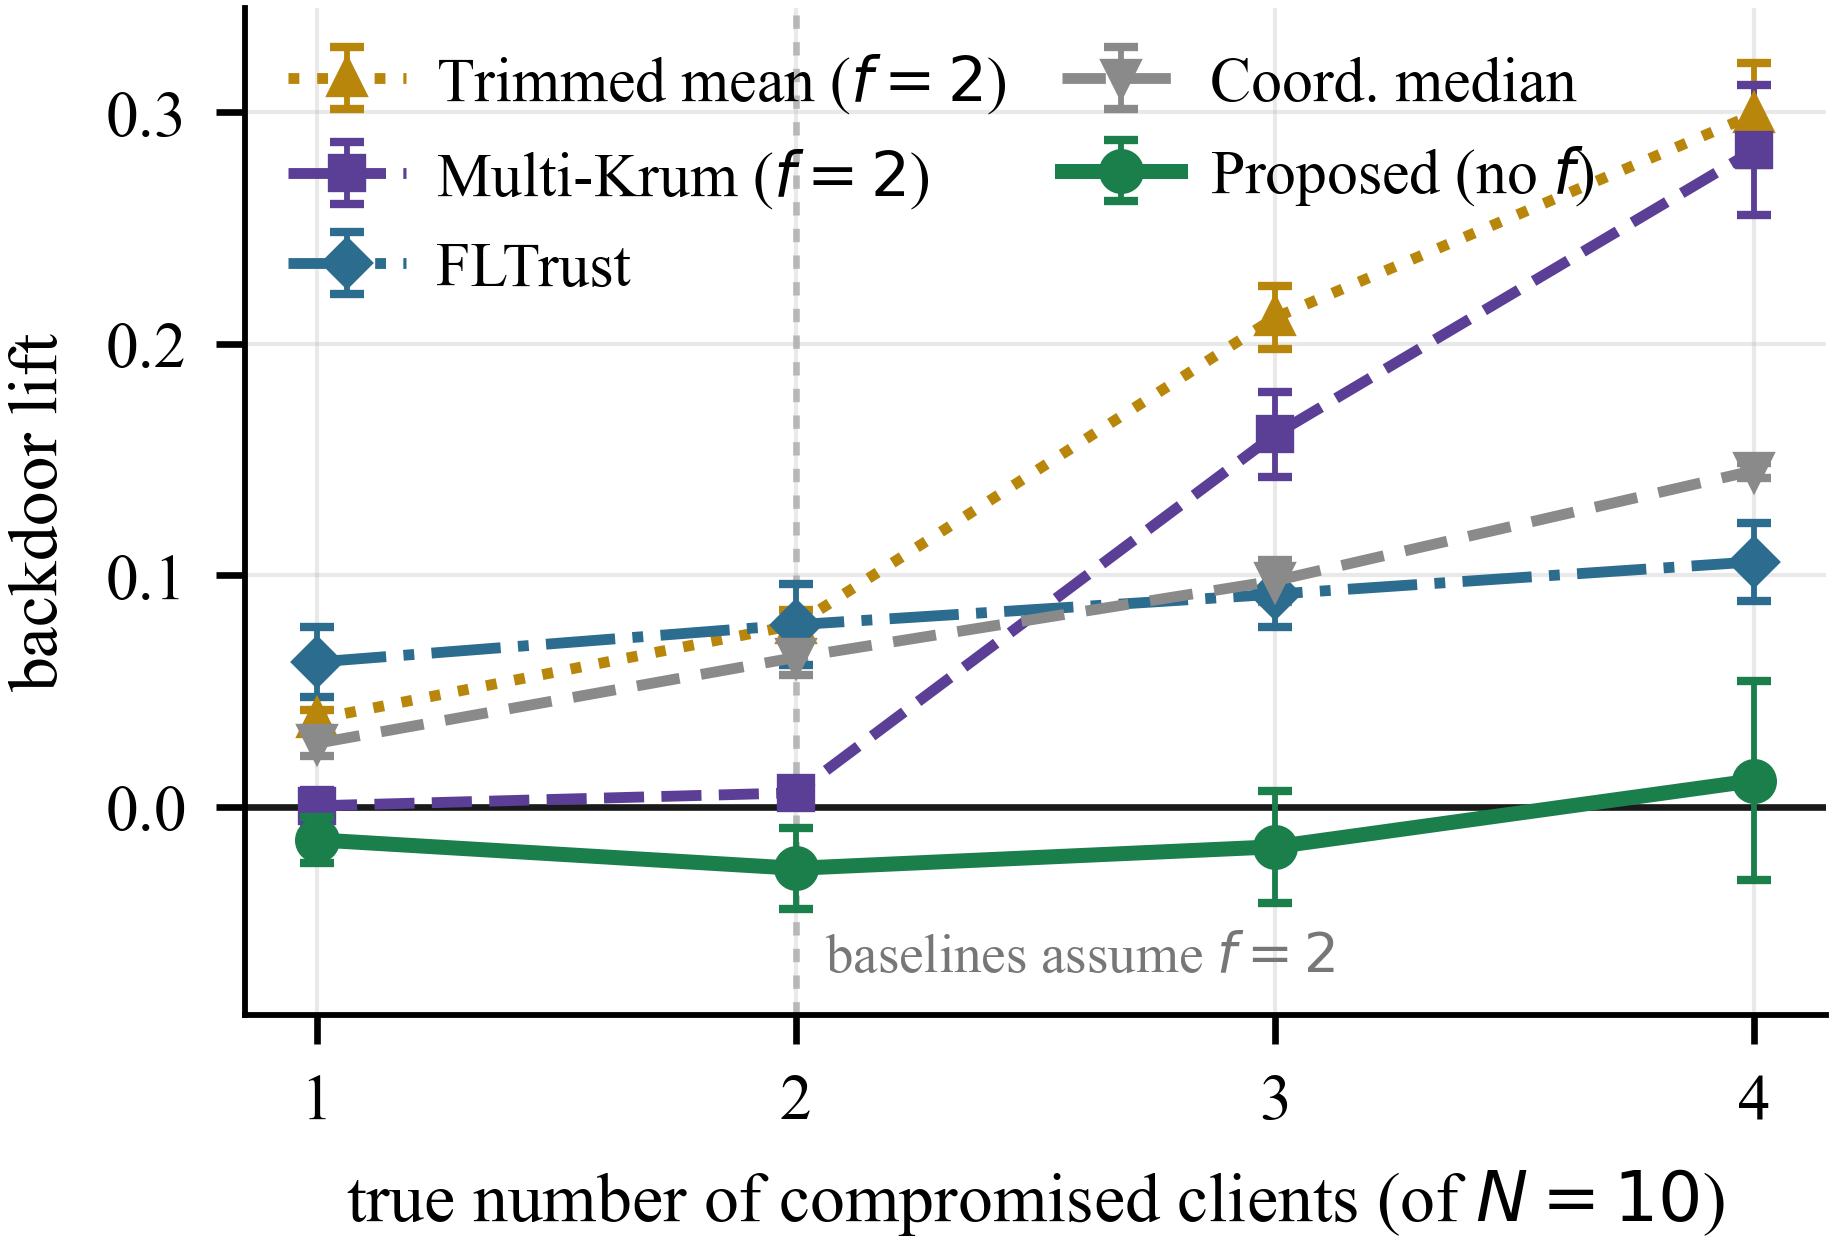
\includegraphics[width=\textwidth]{figures/fig2_fcount.png}
\caption{Backdoor lift as the true number of compromised clients varies while
the Byzantine-robust baselines stay configured for $f=2$ (dashed line). Error
bars are one standard deviation over three seeds.}
\label{fig:fcount}
\end{figure*}

\subsection{Attack Validity and Comparison with Existing Defenses}

\begin{figure*}[!tb]
\centering
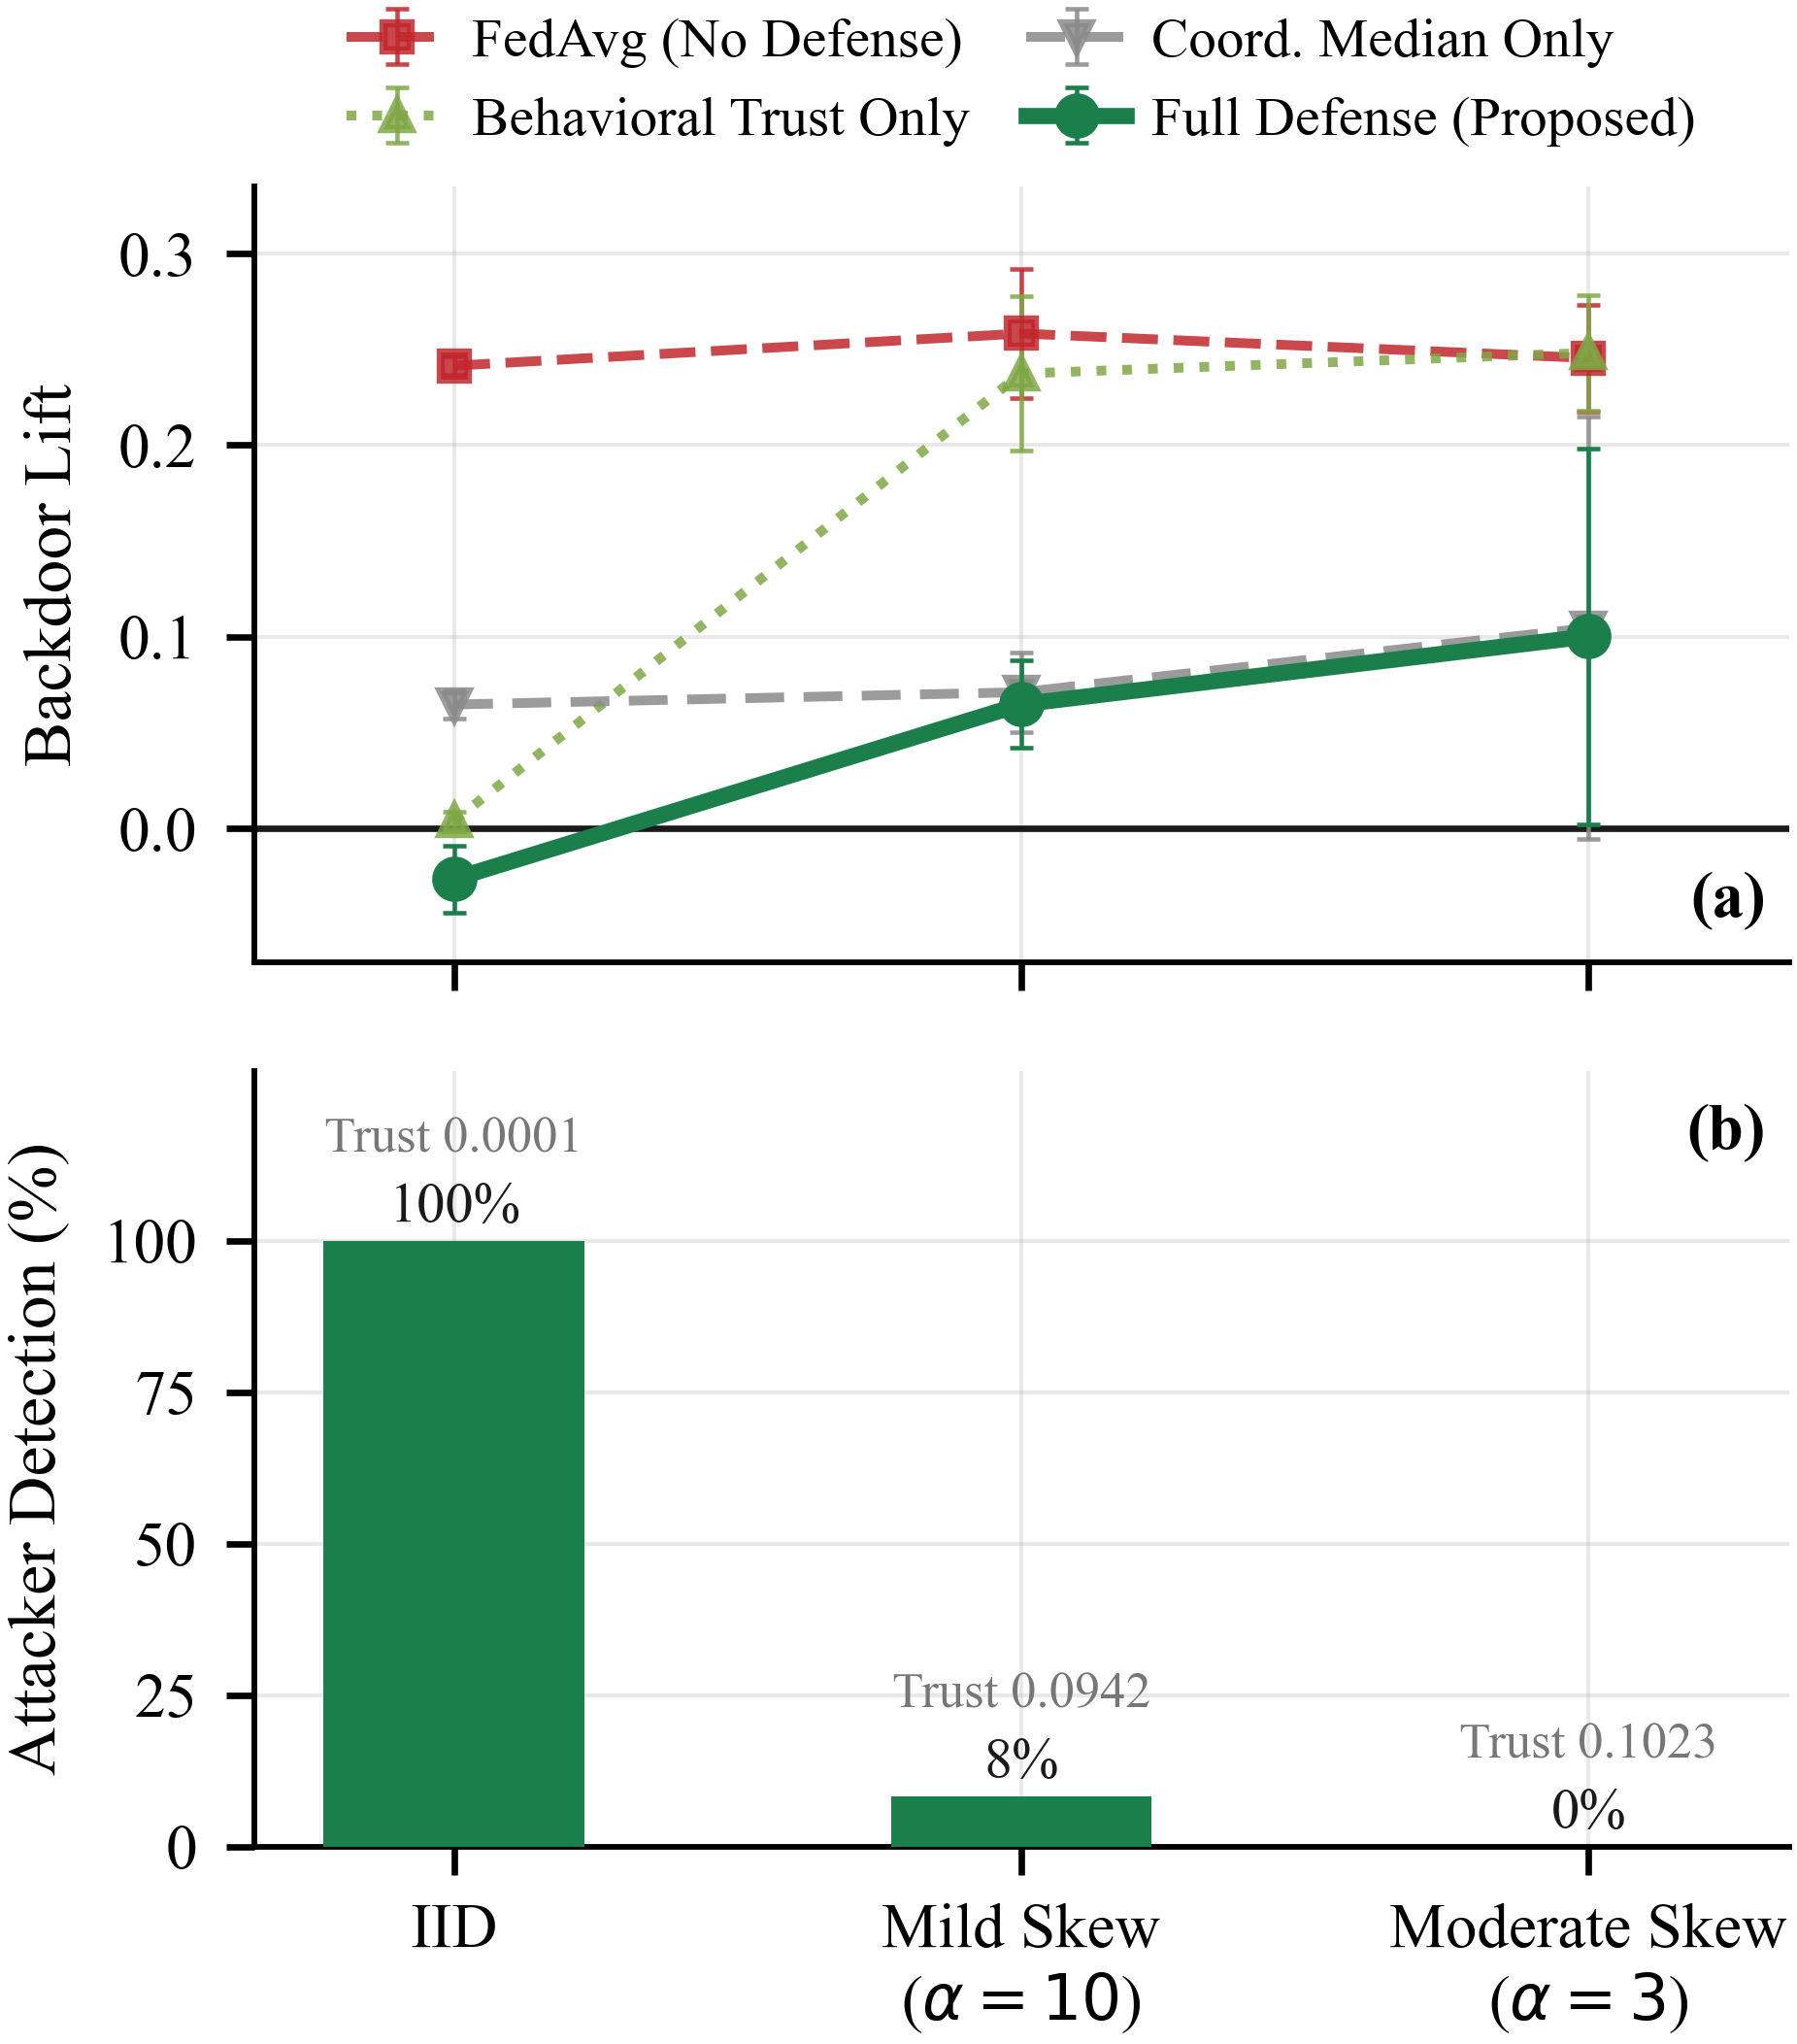
\includegraphics[width=\textwidth]{figures/fig3_noniid.png}
\caption{Effect of client class-ratio skew. (a) Behavioral trust alone
converges toward undefended FedAvg while the full defense tracks the median.
(b) The cause, on twinned axes: attacker trust (right) climbs to the uniform
share exactly as detection (left) collapses.}
\label{fig:noniid}
\end{figure*}

Table~\ref{tab:main} reports every method on the identical split, attack, seeds
and metrics. Four things follow.

The attack is effective and quiet: FedAvg leaves $+0.2415$ of lift while clean
accuracy falls by under two points. Accuracy inflation makes it strictly worse,
$+0.3036$, so a rule consuming an unverified self-report is worse than one
ignoring quality entirely. Median leaves $+0.0646$ and FLTrust $+0.0787$, the
latter with recall \emph{below} the honest baseline because normalizing every
update to the server-update norm throttles honest clients too; it assigns the
attackers $0.039$ trust and flags them in only $84.7\%$ of client-rounds, a
cosine over $3{,}329$ parameters being barely rotated by a small-subspace
backdoor.

\textbf{Multi-Krum is genuinely competitive and we report it as such.} At
$+0.0061$ it is indistinguishable from behavioral trust alone ($+0.0039$) at
far lower cost, so any claim that probing is \emph{necessary} here would be
contradicted by our own table. Krum ($+0.0331$) and trimmed mean ($+0.0787$)
are weaker. What probing adds is attribution (Section~\ref{sec:attrib}) and the
property examined next.



\subsection{Unknown Number of Compromised Clients}

\begin{figure}[!t]
\centering
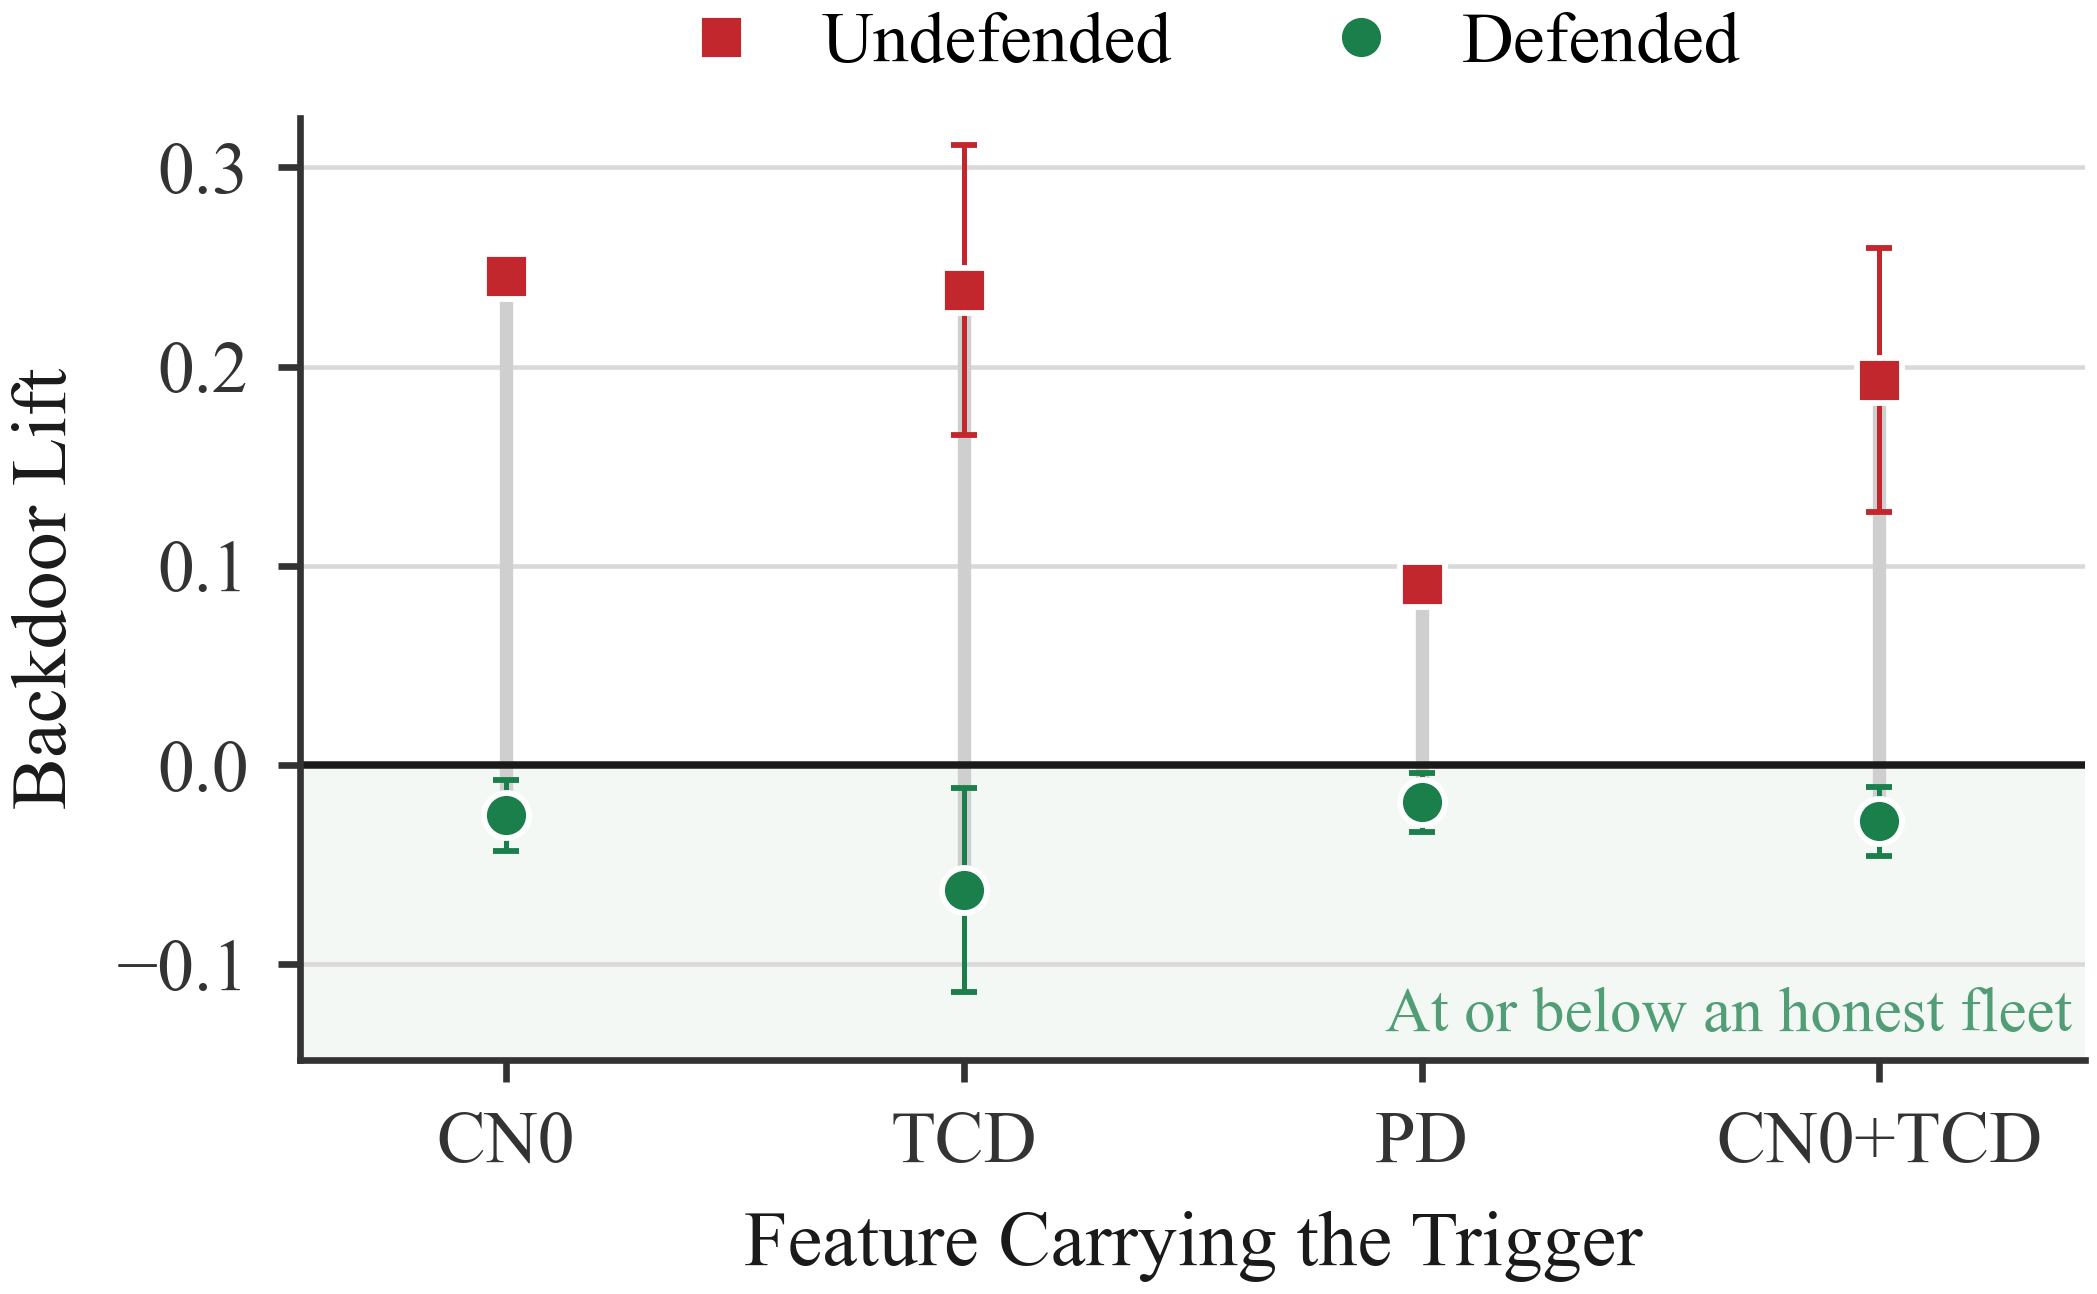
\includegraphics[width=\columnwidth]{figures/fig4_trigger.png}
\caption{Backdoor lift before and after the defense for four trigger settings
under one fixed configuration, never retuned. The shaded band is lift at or
below an honest fleet.}
\label{fig:trigger}
\end{figure}

Table~\ref{tab:main} grants the Byzantine-robust rules an advantage a
deployment cannot: they are told $f$. Fig.~\ref{fig:fcount} varies the true
count from one to four while they stay configured for $f=2$, testing R3
directly. The message is not that Multi-Krum is weak: it reaches $+0.0005$ at
one attacker and $+0.0061$ at two, then degrades to $+0.1609$ at three and
$+0.2837$ at four, close to undefended FedAvg, while trimmed mean reaches
$+0.2992$. The proposed method has no such parameter and stays between
$-0.0265$ and $+0.0114$. Single Krum is a partial exception ($+0.0172$ to
$+0.0331$), since selecting the most central update is insensitive to how many
outliers surround it, at the cost of discarding nine of ten updates per round
and providing no attribution.

\subsection{Client Heterogeneity: Where the Mechanism Stops Working}
\label{sec:noniid}

Eq.~\eqref{eq:susp} assumes honest clients answer the probes similarly.
Fig.~\ref{fig:noniid} tests that by giving clients equal-sized partitions with
unequal benign/spoofed ratios: the realized spoofed fraction spans
$0.19$--$0.59$ at $\alpha=10$ and $0.12$--$0.72$ at $\alpha=3$, against a
global $0.40$. Each condition's honest baseline is retrained, so lift is always
measured against a matched reference.

Under IID the mechanism works as designed: attacker trust $0.0001$ against a
uniform share of $0.100$, detection $100\%$. Under skew it fails. Attacker
trust rises to $0.0942$ then $0.1023$ and detection collapses to $8\%$ then
$0\%$; trust-only aggregation returns $+0.2374$ and $+0.2482$, indistinguishable
from undefended FedAvg on the same partitions. The full defense degrades far
more gracefully, to $+0.0647$ and $+0.1002$, but those track median alone
($+0.0710$, $+0.1046$): under skew the median layer provides essentially all of
the protection.

The cause is the scaling in Eq.~\eqref{eq:susp}. Under IID the cohort is tight,
$\mathrm{MAD}_f$ is small, and a backdoored client's deficit spans many MADs.
Under skew honest clients legitimately disagree, $\mathrm{MAD}_f$ inflates, and
the same absolute deficit becomes a fraction of one MAD: the attacker hides
inside the cohort's own variance. Lowering $\tau$ to $0.5$ recovers detection
only to $38.9\%$ at $\alpha=10$ at a cost of $11.8\%$ honest false flags,
confirming the limitation is the cohort-relative scaling rather than the
threshold. Per-client normalization is the natural remedy, and the median
backstop is retained because it is what survives when the probe does not.


\subsection{Trigger Generalization}

Fig.~\ref{fig:trigger} moves the trigger across features under one fixed
configuration, never retuned, testing R2. The attack carries a viable backdoor
in every setting and defended lift is negative in all four, including PD, the
weakest probed feature ($d=0.152$), and a two-feature CN0$+$TCD trigger not
used in designing the mechanism; DO and LC give $-0.0470$ and $-0.0056$ at the
same configuration. Because a slice exists for every discriminative feature,
relocating the trigger only changes which slice exposes the client. We scope
the claim accordingly: no prior knowledge is needed of which \emph{probed}
feature carries the trigger, and the two features outside $F_{\mathrm{probe}}$
carry too little class separation for a trigger hidden there to be useful.


\subsection{Per-Client Attribution}
\label{sec:attrib}

Byzantine-robust aggregation returns a sanitized model; it does not tell an
operator which aircraft to ground. Behavioral probing scores every client every
round, delivering R4, and the separation over $12$ rounds and three seeds is
categorical: the compromised clients are flagged in $72$ of $72$ attacker
client-rounds at a mean trust of $0.000$, while the eight honest clients sit
between $0.119$ and $0.131$ around the uniform share of $0.100$. One honest
client-round out of $288$ is flagged and none is ever driven to zero trust, so
a false positive down-weights an aircraft for one round rather than silencing
it. The error is asymmetric in the direction a safety-critical deployment
needs.


\subsection{Adaptive Adversary, Root Set, Parameters and Cost}
\label{sec:cost}

Four further studies are summarized here and reported in full in the artifact.
\emph{A defense-aware adversary cannot both hide and keep its backdoor}: an
evasion term of weight $\lambda$ raises mean attacker trust from $0.0001$ to
$0.0834$ at $\lambda=2$, but \emph{undefended} lift falls from $+0.2457$ to
$-0.1433$ and then $-0.4782$ at $\lambda=10$, since the trigger needs a
benign-high input called authentic while evasion trains the same model to call
it spoofed. Defended lift stays negative throughout, between $-0.0253$ and
$-0.0829$. \emph{The root set can be small but must be clean}: shrinking it
tenfold to $600$ rows moves defended lift only to $-0.0276$ at $100\%$
detection, while flipping $30\%$ of its labels drops detection to $83.3\%$, the
expected failure mode for any root-of-trust design including
FLTrust~\cite{cao2021fltrust}. \emph{Parameter sensitivity is mild}: $\beta$
over a sixteen-fold range changes lift by less than one standard deviation, and
$\tau$ has a knee at $2.0$. \emph{Server cost is linear in fleet size}:
$34.0$~ms per round at ten clients, $3.4\%$ of a parallel round, reaching
$34.9\%$ at forty, so we make no large-fleet scalability claim.

\section{Discussion and Conclusion}

Self-reported performance is an exploitable attack surface in federated UAV
spoofing detection: weighting by an unverified client metric is measurably
worse than not weighting at all. Receiver-domain behavioral probing closes that
lever by construction rather than by tuning, and under IID clients reduces
attacker-induced lift to a level indistinguishable from an honest fleet while
naming the compromised aircraft.

We are deliberate about scope. Multi-Krum matches the proposed mechanism in the
nominal IID setting, so the contribution is not a uniformly lower BSR. It is
that the coordinator evaluates clients on evidence it generates itself, without
knowing which probed feature carries the trigger (R2) or how many clients are
compromised (R3), and that it names them (R4) at a $0.3\%$ honest false-flag
rate that never removes a client outright.

Three limitations remain. The evaluation uses one single-receiver dataset as a
proxy for a fleet, so a second signal domain is the strongest possible
validation. Three seeds cannot resolve sub-noise differences between
neighboring defended variants, and we claim none. Finally the base detector is
weak in absolute terms, and the cause is the federated configuration rather
than the dataset: trained centrally the same architecture reaches $0.907$
spoofing recall against $0.529$ federated. That headroom does not distort what
we measure, since lift is paired within seed against an honest run of the
identical configuration, and the trigger is hard for strong models too, the
centrally trained model still calling $37.8\%$ of trigger-bearing samples
authentic. We claim removal of attacker-induced lift, not operational detection
reliability. Replacing the cohort-relative statistic of Eq.~\eqref{eq:susp}
with a per-client normalization is the clearest next step, and
Fig.~\ref{fig:noniid} is the test it must pass. All experiments run through one
shared harness that exports every reported value to CSV, and a single command
reproduces them.

\begin{thebibliography}{00}
\bibitem{mekdad2023survey} Y. Mekdad \emph{et al.}, ``A survey on security and privacy issues of UAVs,'' \emph{Computer Networks}, vol.~224, 2023.
\bibitem{mcmahan2017communication} H.~B. McMahan, E. Moore, D. Ramage, S. Hampson, and B. Ag\"{u}era y Arcas, ``Communication-efficient learning of deep networks from decentralized data,'' in \emph{AISTATS}, 2017, pp.~1273--1282.
\bibitem{udin2025federated} I.~Ud Din, I. Taj, A. Almogren, and M. Guizani, ``Federated learning for trust enhancement in UAV-enabled IoT networks: A unified approach,'' \emph{IEEE Internet Things J.}, vol.~12, no.~8, pp.~9596--9603, 2025.
\bibitem{chai2025navigation} Y. Chai, M. Liu, and M. Li, ``Navigation spoofing and jamming signals identification of UAV based on federated learning,'' \emph{IEEE Internet Things J.}, vol.~12, no.~21, pp.~44177--44188, 2025.
\bibitem{mowla2020federated} N.~I. Mowla, N.~H. Tran, I. Doh, and K. Chae, ``Federated learning-based cognitive detection of jamming attack in flying ad-hoc network,'' \emph{IEEE Access}, vol.~8, pp.~4338--4350, 2020.
\bibitem{bagdasaryan2020backdoor} E. Bagdasaryan, A. Veit, Y. Hua, D. Estrin, and V. Shmatikov, ``How to backdoor federated learning,'' in \emph{AISTATS}, 2020, pp.~2938--2948.
\bibitem{fang2020local} M. Fang, X. Cao, J. Jia, and N.~Z. Gong, ``Local model poisoning attacks to Byzantine-robust federated learning,'' in \emph{USENIX Security}, 2020, pp.~1605--1622.
\bibitem{blanchard2017machine} P. Blanchard, E.~M. El Mhamdi, R. Guerraoui, and J. Stainer, ``Machine learning with adversaries: Byzantine tolerant gradient descent,'' in \emph{NeurIPS}, 2017, pp.~119--129.
\bibitem{cao2021fltrust} X. Cao, M. Fang, J. Liu, and N.~Z. Gong, ``FLTrust: Byzantine-robust federated learning via trust bootstrapping,'' in \emph{NDSS}, 2021.
\bibitem{nguyen2024backdoor} T.~D. Nguyen \emph{et al.}, ``Backdoor attacks and defenses in federated learning: Survey, challenges and future research directions,'' \emph{Eng. Appl. Artif. Intell.}, vol.~127, 2024.
\bibitem{mothukuri2021survey} V. Mothukuri \emph{et al.}, ``A survey on security and privacy of federated learning,'' \emph{Future Gener. Comput. Syst.}, vol.~115, pp.~619--640, 2021.
\bibitem{aissou2022dataset} G. Aissou, ``A dataset for GPS spoofing detection on unmanned aerial system,'' Mendeley Data, V3, 2022, doi:10.17632/z7dj3yyzt8.3.
\bibitem{yin2018byzantine} D. Yin, Y. Chen, K. Ramchandran, and P. Bartlett, ``Byzantine-robust distributed learning: Towards optimal statistical rates,'' in \emph{ICML}, 2018, pp.~5650--5659.
\bibitem{kang2019incentive} J. Kang, Z. Xiong, D. Niyato, S. Xie, and J. Zhang, ``Incentive mechanism for reliable federated learning: A joint optimization approach to combining reputation and contract theory,'' \emph{IEEE Internet Things J.}, vol.~6, no.~6, pp.~10700--10714, 2019.
\bibitem{kairouz2021advances} P. Kairouz \emph{et al.}, ``Advances and open problems in federated learning,'' \emph{Found. Trends Mach. Learn.}, vol.~14, no.~1--2, pp.~1--210, 2021.
\end{thebibliography}

\end{document}
